\documentclass[11pt]{article}
\usepackage[margin=1in]{geometry}\usepackage{amsmath,mathtools,amssymb,amsthm,booktabs,longtable,array,hyperref,graphicx,xcolor}
\hypersetup{colorlinks=true,linkcolor=blue!50!black,urlcolor=blue!50!black}
\newtheorem{thm}{Theorem}
\title{UNNS-U4 Specification, version 001\\Universality and Structural Obstruction Theorems\\for the Reversible SELECT-II Arithmetic Graph}
\author{UNNS Research Collective}\date{10 November 2026}
\begin{document}\maketitle
\begin{abstract}
Let $G$ be the graph on the positive integers with edges $\{kN,k(N+1)^2\}$. We fix the claims a theory of its universality has to settle, with exact hypotheses: (i) which sequences are faithfully coded as marked walks, at what segmentation and routing cost; (ii) which dynamical properties survive the passage to the discrete suspension; (iii) which finite-type systems arise from rules that use only the graph metric, and which cannot (fixed-point dichotomy, real-spectrum obstruction, a triangle-free entropy gap); (iv) what must be declared as additional information. New elementary statements recorded here: finite alphabets embed at cost $\le2$ per transition; the suspension over a symmetric base with a loop has period $1$ or $2$ and period $2$ for every golden-mean embedding; the directed SELECT-II digraph represents no sequence with a descent. The document is a registry of 42 claims with proof dependencies, counterexamples, a correspondence matrix and acceptance gates; it proves nothing beyond U0--U3 except where marked, and records for each claim whether it is already a consequence of earlier releases or needs a new proof.
\end{abstract}
\section{Scope, provenance and reproducibility}
Releases U0--U2, TI, TI-DYN, RN, U3 v001 and U3-COR v001 are unchanged; their hashes are in \texttt{data/provenance\_frozen\_sources.txt} (not re-run, per the project protocol). The frozen records read for \S\ref{sec:corr} are the SELECT-I record (v1.0.0, 21 October 2026, verifier hash $\texttt{cd2f3510}\ldots$ as stated in its \texttt{FREEZE.md}), SELECT-II (v001/v002a/v002b), FIELD-I (v001--v012) and GIG\_I v001, cited through the Master Theorem Registry (Reference Collection v001, commit \texttt{bb8b12d753c6\ldots}, \url{https://github.com/ukbbi/UNNS/tree/bb8b12d753c600c597feb00df17fe139c7cc65fa/projects/UNNS_MATH_FOUNDATIONS/sources}) and the GIG collection (commit \texttt{a115e4bc6b8e\ldots}, \url{https://github.com/ukbbi/UNNS/tree/a115e4bc6b8ee734e6146b3b17a6b121e65d31c3/projects/UNNS_Generative_Information_Geometry}). Nothing in the frozen collection was modified or re-fetched.

\textbf{Reproducibility limitation carried from U3-COR.} The U3-COR verifier located the U3 v001 registration through an absolute path (\texttt{/home/claude/UNNS\_U3}); it therefore runs only on the machine where it was built. This package ships its own copies of the engine files and of the U3 registration record and uses relative paths only; U3-COR itself is not altered.

\section{Vocabulary and the three strengths of universality}
\textbf{Representation} (R): a coding with a decoder; marks, alphabet embedding and routing convention are part of the code. \textbf{Dynamical equivalence} (D): a conjugacy or suspension relation between dynamics. \textbf{Intrinsic structural universality} (I): the structure arises from rules that use only the graph's own isomorphism-invariant data. The registry keeps these separate: a claim classed \emph{intrinsic} may not depend, even transitively, on a non-definitional claim classed representation or additional information (acceptance gate AG3, checked mechanically; see \S\ref{sec:gates}). Every property supplied by markers, embeddings, route tables, observers or controllers is classed as additional information.

\section{Triage: what is already known, what is new}
Of the 42 claims in stages U4.1--U4.6:
\begin{center}\begin{tabular}{@{}lr@{}}\toprule Origin & Claims\\\midrule
consequence of U0--U3 & 3\\
standard theory, specialised & 6\\
new, elementary (proof obligation) & 15\\
frozen record, imported & 9\\
definition & 4\\
open & 5\\
\\\bottomrule\end{tabular}\end{center}
Representation universality (U4.1-T1, T3) and the first-return conjugacy and Abramov relation are consequences of U3 and classical tower theory. The \emph{new} content is elementary but not empty: bounded cost for finite alphabets (using unbounded degree and triangle-freeness), the parity-period theorem, the fixed-point dichotomy and spectral obstructions for metric rules, the triangle-free entropy gap, and the non-universality of the directed digraph. None of the new statements is deep; their value is that they fix the boundary exactly. Five items are open (\S\ref{sec:open}).

\begin{figure}[h]\centering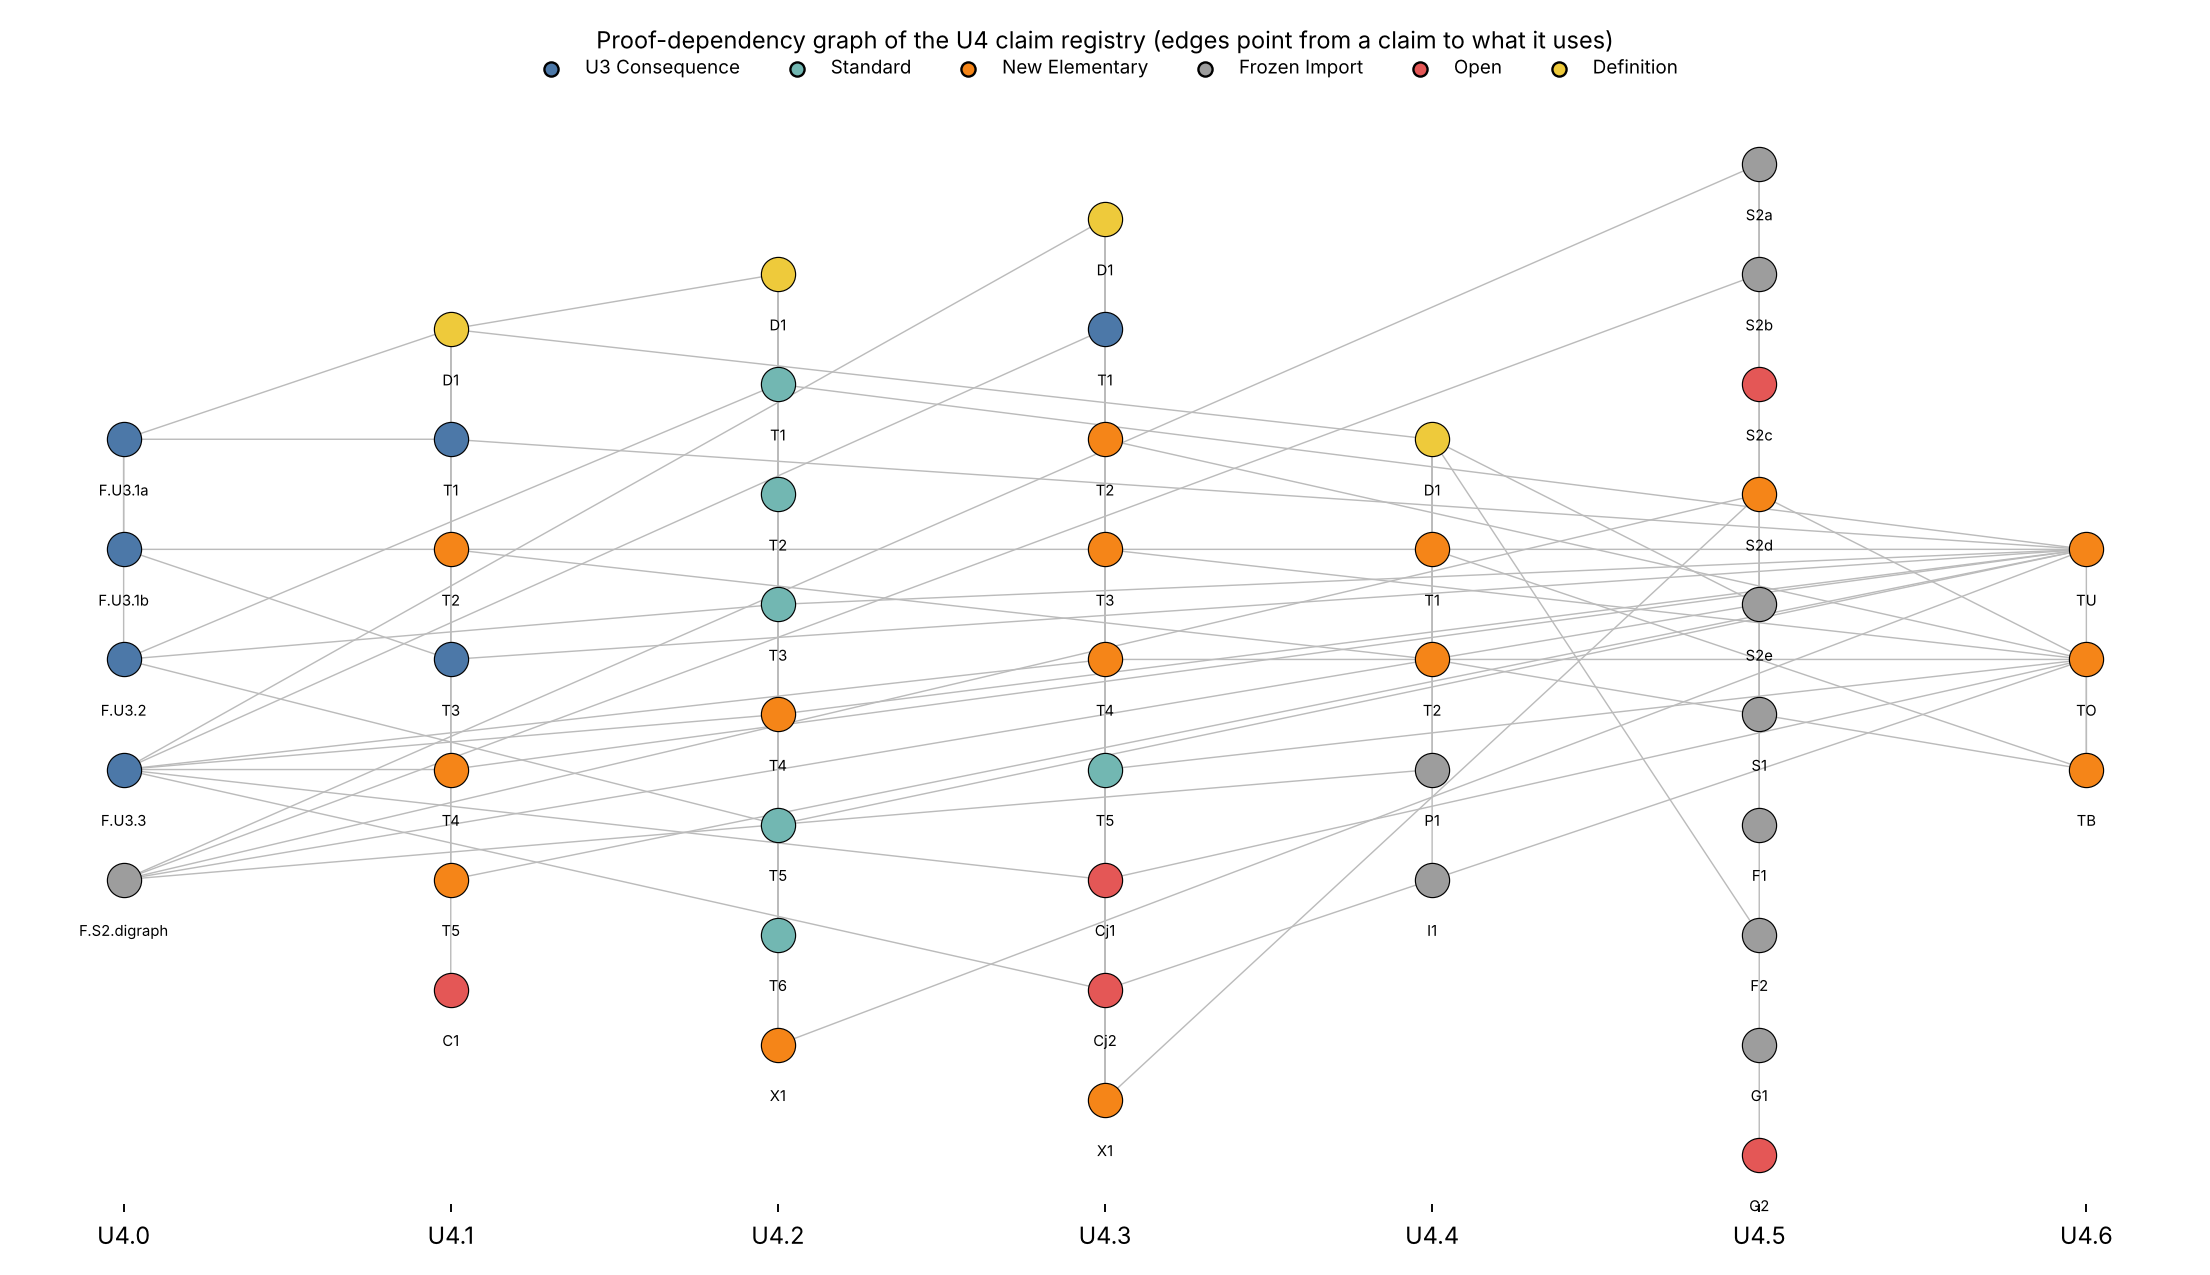
\includegraphics[width=\textwidth]{../figures/dependency_graph.png}
\caption{Proof-dependency graph of the registry, by stage and origin. Orange nodes are new elementary claims whose proofs must be written and independently checked in the U4 body.}\end{figure}

\section{Registry}
\scriptsize
\begin{longtable}{@{}p{1.25cm}p{4.9cm}p{3.0cm}p{3.6cm}p{1.6cm}@{}}\toprule
ID & Title & Origin & Status & Class\\\midrule\endhead
\texttt{F.U3.1a} & Marked universality (U3 v001) & consequence of U0--U3 & Proved (frozen U3 v001) & representation\\
\texttt{F.U3.1b} & Exact segmentation ambiguity (U3-COR) & consequence of U0--U3 & Proved (frozen U3-COR v001) & representation\\
\texttt{F.U3.2} & Suspension facts (U3 v001) & consequence of U0--U3 & Verified-bounded (frozen U3 v001) & representation\\
\texttt{F.U3.3} & Intrinsic admissibility facts (U3 v001) & consequence of U0--U3 & Proved (frozen U3 v001 + COR) & intrinsic\\
\texttt{F.S2.digraph} & SELECT-II digraph facts (S2.1--S2.3, S2.5, S2.10, S2.12) & frozen record, imported & Proved/Checked (frozen SELECT-II) & imported\\
\texttt{U4.1-D1} & Faithful marked-history representation & definition & Definition & representation\\
\texttt{U4.1-T1} & Largest representable class & consequence of U0--U3 & Proved (U3.1a + cardinality) & representation\\
\texttt{U4.1-T2} & Computability transfer & new, elementary (proof obligation) & Sketch (proof obligation PO-1) & representation\\
\texttt{U4.1-T3} & Segmentation information is exact and tight & consequence of U0--U3 & Proved (U3-COR) & representation\\
\texttt{U4.1-T4} & Bounded route cost for finite alphabets & new, elementary (proof obligation) & Sketch + probe (PO-2) & representation\\
\texttt{U4.1-T5} & No bounded cost for infinite alphabets & new, elementary (proof obligation) & Sketch (PO-3) & representation\\
\texttt{U4.1-C1} & Eccentricity growth of the identity embedding & open & Open & representation\\
\texttt{U4.2-D1} & Discrete suspension (Kakutani tower) & definition & Definition & representation\\
\texttt{U4.2-T1} & Return-map conjugacy & standard theory, specialised & Standard (Kakutani); specialisation checked in U3 & representation\\
\texttt{U4.2-T2} & Measure entropy (Abramov) & standard theory, specialised & Standard (Abramov); numerics in U3 agree to $10^{-16}$ & representation\\
\texttt{U4.2-T3} & Topological entropy of the tower & standard theory, specialised & Standard (Bowen / Parry--Pollicott); verified-bounded in U3 & representation\\
\texttt{U4.2-T4} & Parity-period theorem & new, elementary (proof obligation) & Sketch + probe (PO-4) & representation\\
\texttt{U4.2-T5} & Mixing criterion and embedding dependence & standard theory, specialised & Standard criterion + exact certificates (closed sums $5+3+5=13$ odd) & representation\\
\texttt{U4.2-T6} & Recurrence, ergodicity, periodic points & standard theory, specialised & Standard (tower constructions) & representation\\
\texttt{U4.2-X1} & What the suspension does not preserve & new, elementary (proof obligation) & Certificates (recomputed in probe) & representation\\
\texttt{U4.3-D1} & Metric (graph-intrinsic) admissibility rules & definition & Definition & intrinsic\\
\texttt{U4.3-T1} & Structure of $X_r(F)$ & consequence of U0--U3 & Proved (U3 v001) & intrinsic\\
\texttt{U4.3-T2} & Fixed-point dichotomy & new, elementary (proof obligation) & Sketch (PO-5) & intrinsic\\
\texttt{U4.3-T3} & Real-spectrum obstruction (memory 1) & new, elementary (proof obligation) & Sketch + probe (PO-6) & intrinsic\\
\texttt{U4.3-T4} & Triangle-free entropy gap at radius 1 & new, elementary (proof obligation) & Sketch + probe (PO-7) & intrinsic\\
\texttt{U4.3-T5} & Non-SFT systems are excluded & standard theory, specialised & Standard + definition & intrinsic\\
\texttt{U4.3-Cj1} & Finite-graph realisability & open & Open (bounded evidence) & intrinsic\\
\texttt{U4.3-Cj2} & Rigidity and definability cost & open & Open & intrinsic\\
\texttt{U4.3-X1} & Explicit counterexamples to unrestricted intrinsic universality & new, elementary (proof obligation) & Assembled from T2--T5 & intrinsic\\
\texttt{U4.4-D1} & Three tiers and the knowledge ledger & definition & Definition & meta\\
\texttt{U4.4-T1} & Counting bound & new, elementary (proof obligation) & Sketch (PO-8) & additional\\
\texttt{U4.4-T2} & Representation adds no sequence-independent information & new, elementary (proof obligation) & Sketch (PO-9) & additional\\
\texttt{U4.4-P1} & Recognition is intrinsic; scanning order is imported & frozen record, imported & Conditional on frozen statements & imported\\
\texttt{U4.4-I1} & Import obligation: RN negative results & frozen record, imported & Obligation & imported\\
\texttt{U4.5-S2a} & $G$ is the underlying graph of the SELECT-II digraph & frozen record, imported & Proved by definition; probe-checked & imported\\
\texttt{U4.5-S2b} & Degree identity & frozen record, imported & Consequence of frozen S2.1/S2.2; probe $x\le3000$ & imported\\
\texttt{U4.5-S2c} & Orientation is not shown to be intrinsic & open & Open & intrinsic\\
\texttt{U4.5-S2d} & Directed histories are not universal & new, elementary (proof obligation) & Sketch + probe (PO-10) & imported\\
\texttt{U4.5-S2e} & Markov no-go vs marks & frozen record, imported & Conditional on frozen S2.13 & imported\\
\texttt{U4.5-S1} & SELECT-I routes are edges & frozen record, imported & Proved by S2.5; binary part: not addressed & imported\\
\texttt{U4.5-F1} & FIELD-I integer slice & frozen record, imported & Integer slice: consistent; rest: unsupported & imported\\
\texttt{U4.5-F2} & Marks are label recovery, not relational invariants & frozen record, imported & Interpretive; consistent & imported\\
\texttt{U4.5-G1} & GIG history counts vs segmentation counts & frozen record, imported & Unsupported extension (no bridge) & imported\\
\texttt{U4.5-G2} & GIG hierarchy vs U3 ledger & open & Open & imported\\
\texttt{U4.6-TU} & Universality half & new, elementary (proof obligation) & Assembled (new parts: T2, T4, T5, U4.2-T4) & representation\\
\texttt{U4.6-TO} & Obstruction half & new, elementary (proof obligation) & Assembled from U4.3 and U4.5-S2d & intrinsic\\
\texttt{U4.6-TB} & Boundary statement & new, elementary (proof obligation) & Assembled & meta\\
\\\bottomrule\end{longtable}
\normalsize

\section{Exact claims, hypotheses and proof routes}
Statements are given with the hypotheses under which they are intended, the clause that would refute them, and what they use. ``Sketch'' means a proof route is stated but the proof is a U4-body obligation.
\subsection{U4.1 Representational universality}
\paragraph{\texttt{U4.1-D1} --- Faithful marked-history representation.} \emph{Definition; definition; class: representation.} Alphabet $A$ (countable), injection $e:A\to\mathbb N_{>0}$, routing convention $P$, observation marks; \emph{faithful} means a decoder recovers $s$ from $(\iota_e(s),\text{marks})$. \textbf{Hypotheses:} As in U3-0. \textbf{Status:} Definition. \textbf{Refuted by:} n/a. \textbf{Uses:} \texttt{F.U3.1a}.

\paragraph{\texttt{U4.1-T1} --- Largest representable class.} \emph{Theorem; consequence of U0--U3; class: representation.} Marked-history representation exists for sequences (finite, one- or two-sided infinite) over $A$ iff $|A|\le\aleph_0$. No faithful representation exists over an uncountable alphabet. \textbf{Hypotheses:} $e$ injective; sequences of letters, not of real-valued data. \textbf{Proof route:} Sufficiency is U3.1a; necessity: $e$ injective into a countable set. \textbf{Status:} Proved (U3.1a + cardinality). \textbf{Refuted by:} an injection from an uncountable set into $\mathbb N$. \textbf{Uses:} \texttt{U4.1-D1}, \texttt{F.U3.1a}.

\paragraph{\texttt{U4.1-T2} --- Computability transfer.} \emph{Theorem; new, elementary (proof obligation); class: representation.} If $e$ is computable then $s\mapsto\iota_e(s)$ is computable (stream-wise) and $\iota_e(s)\mapsto s$ is computable given the marks; hence $s$ is computable iff its marked history is. The neighbour map is computable (factorisation); feasibility beyond the certification bound ($3.3\times10^{24}$) is a separate, experimental level. \textbf{Hypotheses:} Exact integer arithmetic; certification policy RN-0. \textbf{Proof route:} BFS balls are finite (local finiteness), so $d_G$ and $P$ are computable. \textbf{Status:} Sketch (proof obligation PO-1). \textbf{Refuted by:} a computable $s$ with non-computable $\iota_e(s)$ for computable $e$. \textbf{Uses:} \texttt{U4.1-D1}, \texttt{F.U3.1b}.

\paragraph{\texttt{U4.1-T3} --- Segmentation information is exact and tight.} \emph{Theorem; consequence of U0--U3; class: representation.} Unmarked walks need $\lceil\log_2M(w)\rceil\le L-1$ extra bits to decode, and $L-1$ bits are necessary for some walks of every length. \textbf{Hypotheses:} Same as F.U3.1b. \textbf{Status:} Proved (U3-COR). \textbf{Refuted by:} see F.U3.1b. \textbf{Uses:} \texttt{F.U3.1b}.

\paragraph{\texttt{U4.1-T4} --- Bounded route cost for finite alphabets.} \emph{Theorem; new, elementary (proof obligation); class: representation.} For every $k\ge3$ there is an embedding of a $k$-letter alphabet with all pairwise distances $\le2$ (a vertex $x$ with $\deg x\ge k-1$ and $k-1$ of its neighbours), so every transition costs at most $2$ steps (repeats cost $2$ by convention). Minimal such radius: $r^*(2)=1$, $r^*(k)=2$ for $k\ge3$. \textbf{Hypotheses:} $\tau(x)\le\deg x$ unbounded; $G$ triangle-free (gives $r^*(3)\ge2$). \textbf{Proof route:} $\tau(x)\to\infty$; closed neighbourhood of $x$ has diameter $\le2$; triangle-free excludes radius 1 for $k\ge3$. \textbf{Status:} Sketch + probe (PO-2). \textbf{Refuted by:} a $k$ for which no vertex of degree $\ge k-1$ exists, or three vertices pairwise adjacent. \textbf{Uses:} \texttt{F.U3.3}, \texttt{U4.1-D1}. \textbf{Probe:} P1.

\paragraph{\texttt{U4.1-T5} --- No bounded cost for infinite alphabets.} \emph{Theorem; new, elementary (proof obligation); class: representation.} If $A$ is infinite and $e$ injective then $\sup_{a,b}d_G(e(a),e(b))=\infty$; hence the full shift over an infinite alphabet has unbounded roof. \textbf{Hypotheses:} $G$ locally finite. \textbf{Proof route:} Balls of finite radius are finite. \textbf{Status:} Sketch (PO-3). \textbf{Refuted by:} an infinite subset of $V$ of bounded diameter. \textbf{Uses:} \texttt{U4.1-D1}.

\paragraph{\texttt{U4.1-C1} --- Eccentricity growth of the identity embedding.} \emph{Conjecture; open; class: representation.} Growth rate of $\max_{n\le N}d_G(1,n)$ is unknown; trivially $\le6(N-1)$ from bounded successor distance; no data or rate is claimed. \textbf{Hypotheses:} Frozen U1-BND ($\sup d(n,n+1)=6$). \textbf{Status:} Open. \textbf{Refuted by:} a proof or counterexample of any specified rate. \textbf{Uses:} \texttt{U4.1-D1}.

\subsection{U4.2 Dynamical correspondence}
\paragraph{\texttt{U4.2-D1} --- Discrete suspension (Kakutani tower).} \emph{Definition; definition; class: representation.} Base $(X,\sigma)$ a subshift over $A$ with embedding $e$; roof $r(s)=d_G(e(s_0),e(s_1))$ ($=2$ if $s_0=s_1$); tower $\{(s,j):0\le j<r(s)\}$ with the primitive successor map. \textbf{Hypotheses:} $r$ depends on two coordinates and is a positive integer; bounded when $A$ finite. \textbf{Status:} Definition. \textbf{Refuted by:} n/a. \textbf{Uses:} \texttt{U4.1-D1}.

\paragraph{\texttt{U4.2-T1} --- Return-map conjugacy.} \emph{Theorem; standard theory, specialised; class: representation.} The first-return map of the tower to the base section $\{j=0\}$ is conjugate to $\sigma$. \textbf{Hypotheses:} As in D1. \textbf{Status:} Standard (Kakutani); specialisation checked in U3. \textbf{Refuted by:} a sequence whose first return is not $\sigma(s)$. \textbf{Uses:} \texttt{U4.2-D1}, \texttt{F.U3.2}.

\paragraph{\texttt{U4.2-T2} --- Measure entropy (Abramov).} \emph{Theorem; standard theory, specialised; class: representation.} For ergodic $\mu$ with $\bar r=\int r\,d\mu<\infty$: $h_{\mu^r}=h_\mu/\bar r$. \textbf{Hypotheses:} Ergodic $\mu$, finite mean roof. \textbf{Status:} Standard (Abramov); numerics in U3 agree to $10^{-16}$. \textbf{Refuted by:} a Markov measure with $h_{\mu^r}\ne h_\mu/\bar r$. \textbf{Uses:} \texttt{U4.2-D1}, \texttt{U4.2-T1}.

\paragraph{\texttt{U4.2-T3} --- Topological entropy of the tower.} \emph{Theorem; standard theory, specialised; class: representation.} For an irreducible 1-step SFT base with transition matrix $B$ and two-coordinate roof, $h_{top}$ of the tower is $\log\lambda$ with $\lambda>1$ the largest solution of $\rho\big(B\circ[\lambda^{-r(a,b)}]\big)=1$ (pressure equation $P(-h\,r)=0$). Golden mean: $1-w-w^{d}=0$, $w=\lambda^{-2}$. In general $h_{top}\ge h_\mu/\bar r$ for every ergodic $\mu$; equality for the Parry measure is \emph{not} asserted beyond the golden-mean $(2,d,d)$ family, where it holds iff $d=2$. \textbf{Hypotheses:} Irreducible SFT base; the general `iff constant roof' claim is withdrawn (U3-COR). \textbf{Status:} Standard (Bowen / Parry--Pollicott); verified-bounded in U3. \textbf{Refuted by:} an embedding whose expanded-graph entropy differs from the root of the renewal equation. \textbf{Uses:} \texttt{U4.2-D1}, \texttt{U4.2-T2}, \texttt{F.U3.2}. \textbf{Probe:} P6.

\paragraph{\texttt{U4.2-T4} --- Parity-period theorem.} \emph{Theorem; new, elementary (proof obligation); class: representation.} Let the base pair relation be symmetric and let an irreducible component $C$ contain a self-transition. Then the period of the tower over $C$ is $1$ or $2$, and equals $2$ iff there is $f:C\to\mathbb Z/2$ with $d_G(a,b)\equiv f(a)+f(b)\pmod 2$ on every allowed pair $a\ne b$. In particular the golden-mean tower has period $2$ for \emph{every} embedding. \textbf{Hypotheses:} Symmetric base relation; at least one loop (roof $2$) in $C$. \textbf{Proof route:} The loop gives closed sum $2$, so period divides $2$; all closed sums even iff a parity potential exists. Golden mean: $f(0)=0$, $f(1)=d\bmod2$. \textbf{Status:} Sketch + probe (PO-4). \textbf{Refuted by:} a symmetric base component with a loop whose tower period is $>2$, or a golden-mean embedding of period $1$. \textbf{Uses:} \texttt{U4.2-D1}, \texttt{F.U3.3}. \textbf{Probe:} P2,P6.

\paragraph{\texttt{U4.2-T5} --- Mixing criterion and embedding dependence.} \emph{Theorem; standard theory, specialised; class: representation.} If the base is an irreducible aperiodic SFT, the tower is topologically mixing iff its period is $1$. Mixing of the tower is therefore a property of $(\text{base},e)$, not of the base alone: for the 3-letter full shift, $\{1,2,3\}$ gives period $2$ while $\{1,2,5\}$ gives period $1$. \textbf{Hypotheses:} Irreducible aperiodic SFT base. \textbf{Status:} Standard criterion + exact certificates (closed sums $5+3+5=13$ odd). \textbf{Refuted by:} recomputed distances not equal to $5,3,5$ for $\{1,2,5\}$. \textbf{Uses:} \texttt{U4.2-T4}, \texttt{F.U3.2}. \textbf{Probe:} P6.

\paragraph{\texttt{U4.2-T6} --- Recurrence, ergodicity, periodic points.} \emph{Theorem; standard theory, specialised; class: representation.} A base periodic orbit with roof sum $R$ yields a tower periodic orbit of period $R$; the tower measure is ergodic iff the base measure is; Poincar\'e recurrence holds for finite tower measure ($\bar r<\infty$). \textbf{Hypotheses:} As in D1; $\bar r<\infty$. \textbf{Status:} Standard (tower constructions). \textbf{Refuted by:} a tower periodic point not arising from a base cycle. \textbf{Uses:} \texttt{U4.2-D1}, \texttt{U4.2-T1}.

\paragraph{\texttt{U4.2-X1} --- What the suspension does not preserve.} \emph{Proposition; new, elementary (proof obligation); class: representation.} (i) entropy $h_{top}$ of the tower depends on $e$ (golden mean: $d=2$ vs $d=5$ give $0.2406$ vs $0.1406$), so towers over the same base can be non-conjugate; (ii) period and mixing depend on $e$ (T5); (iii) $h_{top}\neq h_{top}(\text{base})/\bar r$ in general. \textbf{Hypotheses:} Explicit certificates. \textbf{Status:} Certificates (recomputed in probe). \textbf{Refuted by:} two embeddings with equal data but different entropy. \textbf{Uses:} \texttt{U4.2-T3}, \texttt{U4.2-T5}. \textbf{Probe:} P6.

\subsection{U4.3 Intrinsic admissibility and obstruction}
\paragraph{\texttt{U4.3-D1} --- Metric (graph-intrinsic) admissibility rules.} \emph{Definition; definition; class: intrinsic.} A rule of memory $m$ on a finite window $F\subset V$ is a predicate $\Phi$ on $(m{+}1)$-tuples that depends only on the matrix $(d_G(x_i,x_j))_{i,j\le m}$; $X_\Phi(F)$ = sequences all of whose $(m{+}1)$-blocks satisfy $\Phi$. $X_r(F)$ is $m=1$, $\Phi=[d\le r]$. \textbf{Hypotheses:} Finite $F$, finite memory. \textbf{Status:} Definition. \textbf{Refuted by:} n/a. \textbf{Uses:} \texttt{F.U3.3}.

\paragraph{\texttt{U4.3-T1} --- Structure of $X_r(F)$.} \emph{Theorem; consequence of U0--U3; class: intrinsic.} $X_r(F)$ is a 1-step SFT whose pair relation is reflexive and symmetric; fixed points $=|F|$. \textbf{Hypotheses:} As in D1. \textbf{Status:} Proved (U3 v001). \textbf{Refuted by:} a non-symmetric or non-reflexive pair relation. \textbf{Uses:} \texttt{U4.3-D1}, \texttt{F.U3.3}.

\paragraph{\texttt{U4.3-T2} --- Fixed-point dichotomy.} \emph{Theorem; new, elementary (proof obligation); class: intrinsic.} For every metric rule $\Phi$ of any memory $m$ on a finite $F$: the number of fixed points of $X_\Phi(F)$ is $0$ or $|F|$. Hence a target SFT with $f\ge1$ fixed points is conjugate to a metric-rule shift only on exactly $f$ letters, all of them constants. The golden-mean shift ($f=1$, entropy $\log\varphi$) is conjugate to none. \textbf{Hypotheses:} Finite $F$; $m<\infty$; conjugacy preserves fixed points. \textbf{Proof route:} Every constant window $(x,\dots,x)$ has the zero distance matrix, so its admissibility does not depend on $x$. \textbf{Status:} Sketch (PO-5). \textbf{Refuted by:} a metric rule with a constant accepted for some letters but not others. \textbf{Uses:} \texttt{U4.3-D1}.

\paragraph{\texttt{U4.3-T3} --- Real-spectrum obstruction (memory 1).} \emph{Theorem; new, elementary (proof obligation); class: intrinsic.} A memory-1 metric shift has a symmetric transition matrix, hence real spectrum; the sequence $p_n=\operatorname{tr}B^n$ of periodic-point counts determines the nonzero spectrum, so an SFT with a non-real nonzero eigenvalue is not conjugate to any memory-1 metric shift. Example: the 3-cycle with loops, $B=\begin{psmallmatrix}1&1&0\\0&1&1\\1&0&1\end{psmallmatrix}$, spectrum $\{2,1+\omega,1+\bar\omega\}$. \textbf{Hypotheses:} Memory 1 only; memory $\ge2$ rules may be asymmetric --- OPEN. \textbf{Proof route:} Newton identities recover the nonzero spectrum from $(\operatorname{tr}B^n)_n$. \textbf{Status:} Sketch + probe (PO-6). \textbf{Refuted by:} a symmetric matrix with the same $\operatorname{tr}B^n$ as $B$. \textbf{Uses:} \texttt{U4.3-D1}, \texttt{U4.3-T1}. \textbf{Probe:} P3.

\paragraph{\texttt{U4.3-T4} --- Triangle-free entropy gap at radius 1.} \emph{Theorem; new, elementary (proof obligation); class: intrinsic.} For $k\ge3$ the full $k$-shift is not conjugate to any $X_1(F)$: conjugacy forces $|F|=k$ (T2), the pair graph is triangle-free (F.U3.3), and $\rho(A+I)=1+\rho(A)\le1+\sqrt{m}\le1+k/2<k$ (Nosal; Mantel). For radius 2 the full $k$-shift is realised by a star (U4.1-T4). \textbf{Hypotheses:} Finite $F$. \textbf{Proof route:} Classical inputs: Mantel (edge bound), Nosal (spectral bound) --- prior-art review pending. \textbf{Status:} Sketch + probe (PO-7). \textbf{Refuted by:} a triangle-free graph on $k$ vertices with $\rho(A+I)\ge k$. \textbf{Uses:} \texttt{U4.3-T2}, \texttt{F.U3.3}. \textbf{Probe:} P3.

\paragraph{\texttt{U4.3-T5} --- Non-SFT systems are excluded.} \emph{Proposition; standard theory, specialised; class: intrinsic.} Being an SFT is a conjugacy invariant; every $X_\Phi(F)$ is an SFT; hence no non-SFT subshift (e.g.\ the even shift, Sturmian shifts) is conjugate to a finite-memory metric shift. Rules with unbounded memory are outside the class. \textbf{Hypotheses:} Finite memory. \textbf{Status:} Standard + definition. \textbf{Refuted by:} a finite-memory metric shift that is not an SFT. \textbf{Uses:} \texttt{U4.3-D1}.

\paragraph{\texttt{U4.3-Cj1} --- Finite-graph realisability.} \emph{Conjecture; open; class: intrinsic.} Every finite graph is an induced subgraph of $G^{(r)}$ (vertices adjacent iff $d_G\le r$) for some $r$. If true, every reflexive symmetric memory-1 SFT with loops everywhere is $X_r(F)$ for some $r$. \textbf{Hypotheses:} Bounded evidence only: 30/30 connected graphs on $\le5$ vertices at $r=2,3$; $K_{2,3}$ not found at $r=1$ (U3 v001). \textbf{Status:} Open (bounded evidence). \textbf{Refuted by:} a finite graph not embeddable at any $r$ (needs proof); a $\le6$-vertex graph failing at $r\le3$ within bounds. \textbf{Uses:} \texttt{F.U3.3}.

\paragraph{\texttt{U4.3-Cj2} --- Rigidity and definability cost.} \emph{Conjecture; open; class: intrinsic.} $\mathrm{Aut}(G)$ is trivial. If so, every vertex is definable from the graph (vertex $1$ is the unique vertex of degree $1$), and `naming' a vertex costs its description length --- the formal price of leaving the metric-rule class. \textbf{Hypotheses:} Local probe is inconclusive: degree-coloured balls of radius 2, 3 have a nontrivial automorphism group of order 2 (boundary symmetry only). \textbf{Status:} Open. \textbf{Refuted by:} a nontrivial automorphism of $G$. \textbf{Uses:} \texttt{F.U3.3}. \textbf{Probe:} P7.

\paragraph{\texttt{U4.3-X1} --- Explicit counterexamples to unrestricted intrinsic universality.} \emph{Proposition; new, elementary (proof obligation); class: intrinsic.} (a) golden mean (T2); (b) the 3-cycle with loops (T3); (c) full $k$-shift ($k\ge3$) at $r=1$ (T4); (d) any non-SFT (T5); (e) the \emph{directed} SELECT-II digraph represents no sequence with a descent (U4.5-S2d). Each is a theorem about the stated class, not about every conceivable intrinsic grammar. \textbf{Hypotheses:} Classes as stated. \textbf{Status:} Assembled from T2--T5. \textbf{Refuted by:} a missing hypothesis in any component. \textbf{Uses:} \texttt{U4.3-T2}, \texttt{U4.3-T3}, \texttt{U4.3-T4}, \texttt{U4.3-T5}, \texttt{U4.5-S2d}.

\subsection{U4.4 Generative information boundary}
\paragraph{\texttt{U4.4-D1} --- Three tiers and the knowledge ledger.} \emph{Definition; definition; class: meta.} \emph{Representation}: a coding with decoder. \emph{Finite-control generation}: a program of $K$ declared bits that drives graph moves. \emph{Intrinsic generation}: no sequence-specific input; the orbit is determined by graph structure (and the start vertex). Ledger: $L(s)$ steps, $M(s)$ segmentation bits, $C_{route}$, $C_{cert}$, $K(e,P)$ reported separately. \textbf{Hypotheses:} As in U3 cost ledger. \textbf{Status:} Definition. \textbf{Refuted by:} n/a. \textbf{Uses:} \texttt{U4.1-D1}.

\paragraph{\texttt{U4.4-T1} --- Counting bound.} \emph{Theorem; new, elementary (proof obligation); class: additional.} A generator with $K$ declared bits produces at most $2^{K+1}-1$ distinct sequences; to cover all $2^n$ words over two letters one needs $K\ge n-1$. Only countably many sequences are produced by any fixed-program intrinsic dynamics (one orbit per start vertex). \textbf{Hypotheses:} Deterministic generators. \textbf{Status:} Sketch (PO-8). \textbf{Refuted by:} a generator with fewer than $n-1$ bits producing all $2^n$ words. \textbf{Uses:} \texttt{U4.4-D1}.

\paragraph{\texttt{U4.4-T2} --- Representation adds no sequence-independent information.} \emph{Theorem; new, elementary (proof obligation); class: additional.} $K(\iota_e(s))=K(s)+O(1)$, with the constant depending only on the fixed program for $G$, $P$, $e$. A sequence-specific route table has at least the complexity of the sequence. \textbf{Hypotheses:} Fixed computable $e$; prefix complexity. \textbf{Proof route:} Invariance theorem for Kolmogorov complexity; two computable maps. \textbf{Status:} Sketch (PO-9). \textbf{Refuted by:} a sequence whose marked history is simpler than the sequence by more than $O(1)$. \textbf{Uses:} \texttt{U4.1-T2}, \texttt{U4.4-D1}.

\paragraph{\texttt{U4.4-P1} --- Recognition is intrinsic; scanning order is imported.} \emph{Proposition; frozen record, imported; class: imported.} The predicate `$p$ prime $\iff\deg(p)=2$' is intrinsic to $G$. Listing the primes by scanning $\mathbb N$ with a bounded successor route and filtering by degree uses an imported enumeration of $V$ (finite control, $O(1)$ declared bits, certification cost $C_{cert}$ large); it is finite-control generation, not intrinsic generation. \textbf{Hypotheses:} Frozen TI-DYN degree--primality theorem and U1-BND bounded successor distance as recorded; not re-derived here. \textbf{Status:} Conditional on frozen statements. \textbf{Refuted by:} a prime of degree $\ne2$ or a non-prime of degree 2. \textbf{Uses:} \texttt{U4.4-D1}, \texttt{F.S2.digraph}. \textbf{Probe:} P8.

\paragraph{\texttt{U4.4-I1} --- Import obligation: RN negative results.} \emph{Gate; frozen record, imported; class: imported.} RN v001 classification of ranked-neighbour trajectories (stuck, divergent, prime visits) is imported with hashes in the U4 body; none of it is restated here. \textbf{Hypotheses:} \texttt{NOT\_RERUN}; hash-preserved. \textbf{Status:} Obligation. \textbf{Refuted by:} hash mismatch of the RN release. \textbf{Uses:} \texttt{U4.4-D1}.

\subsection{U4.5 SELECT / FIELD / GIG correspondence}
\paragraph{\texttt{U4.5-S2a} --- $G$ is the underlying graph of the SELECT-II digraph.} \emph{Proposition; frozen record, imported; class: imported.} The edge set $\{kN,k(N+1)^2\}$ of $G$ equals the set of SELECT-II arrows $m\to m(N+1)^2/N$, $N\mid m$, forgetting orientation. \textbf{Hypotheses:} Frozen SELECT-II v001 definition. \textbf{Status:} Proved by definition; probe-checked. \textbf{Refuted by:} a pair $(m,t)$ adjacent in one and not the other. \textbf{Uses:} \texttt{F.S2.digraph}. \textbf{Probe:} P4.

\paragraph{\texttt{U4.5-S2b} --- Degree identity.} \emph{Proposition; frozen record, imported; class: imported.} $\deg x=\tau(x)+R(x)$, $R(x)=\#\{d\ge2:d^2\mid x\}$ (outdegree + indegree). \textbf{Hypotheses:} S2.1, S2.2. \textbf{Status:} Consequence of frozen S2.1/S2.2; probe $x\le3000$. \textbf{Refuted by:} an $x$ with $\deg x\ne\tau+R$. \textbf{Uses:} \texttt{U4.5-S2a}, \texttt{F.S2.digraph}. \textbf{Probe:} P8.

\paragraph{\texttt{U4.5-S2c} --- Orientation is not shown to be intrinsic.} \emph{Conjecture; open; class: intrinsic.} Whether the orientation (increasing direction) of the SELECT-II digraph can be recovered from the unlabelled graph $G$ alone is open; the integer order is used in the frozen definition. \textbf{Status:} Open. \textbf{Refuted by:} an isomorphism-invariant rule recovering orientation (or a proof that none exists). \textbf{Uses:} \texttt{U4.5-S2a}.

\paragraph{\texttt{U4.5-S2d} --- Directed histories are not universal.} \emph{Theorem; new, elementary (proof obligation); class: imported.} In the SELECT-II digraph every arrow multiplies by $\ge4$, so the digraph is acyclic and a directed waypoint sequence is strictly increasing. No sequence with a descent (e.g.\ $2,1$) is a waypoint sequence of a directed history. Universality of U3 is a property of the \emph{reversible} graph $G$ (inverse moves), not of SELECT-II's native dynamics. \textbf{Hypotheses:} Frozen S2.1. \textbf{Proof route:} Growth factor $N+2+1/N\ge4$. \textbf{Status:} Sketch + probe (PO-10). \textbf{Refuted by:} a directed path from $m$ to $t<m$. \textbf{Uses:} \texttt{F.S2.digraph}, \texttt{U4.5-S2a}. \textbf{Probe:} P5.

\paragraph{\texttt{U4.5-S2e} --- Markov no-go vs marks.} \emph{Proposition; frozen record, imported; class: imported.} Frozen S2.13 (continuations depend on the endpoint only) is consistent with U3: memory beyond the endpoint lives entirely in the marks, i.e.\ in declared information. \textbf{Hypotheses:} S2.13. \textbf{Status:} Conditional on frozen S2.13. \textbf{Refuted by:} a continuation rule using history without marks. \textbf{Uses:} \texttt{F.S2.digraph}, \texttt{U4.4-D1}.

\paragraph{\texttt{U4.5-S1} --- SELECT-I routes are edges.} \emph{Proposition; frozen record, imported; class: imported.} SELECT-I anchor routes $(k,d)$ with value $kd^2$ correspond to edges $k(d-1)\to kd^2$ (frozen S2.5). SELECT-I's binary continuation/join questions ($J_{\mathrm{join}}$, $J_{\mathrm{ref}}$) concern a \emph{binary} structure; the unary graph $G$ carries none, and U3/U4 claim nothing about it. \textbf{Hypotheses:} Frozen SELECT-I v1.0.0, S2.5. \textbf{Status:} Proved by S2.5; binary part: not addressed. \textbf{Refuted by:} a route not equal to an edge. \textbf{Uses:} \texttt{U4.5-S2a}.

\paragraph{\texttt{U4.5-F1} --- FIELD-I integer slice.} \emph{Proposition; frozen record, imported; class: imported.} Frozen F.T1 with $b=1$: occurrences of the integer $a$ are $\{d\ge2:d^2\mid a\}$, of size $R(a)=\operatorname{indeg}(a)$. Rational (non-anchor) outputs, the collective operator $C(x)=x+L^2/G$ and all FIELD dynamics are \emph{not} represented in $G$ (unsupported extension). \textbf{Hypotheses:} Frozen FIELD-I v001--v012 as recorded. \textbf{Status:} Integer slice: consistent; rest: unsupported. \textbf{Refuted by:} integer fibre size $\ne R(a)$. \textbf{Uses:} \texttt{U4.5-S2b}. \textbf{Probe:} P4.

\paragraph{\texttt{U4.5-F2} --- Marks are label recovery, not relational invariants.} \emph{Proposition; frozen record, imported; class: imported.} FIELD-I's leakage criterion (label recovery alone fails the nontrivial-invariant criterion) classifies the U3 decoder as \emph{representation}: it recovers labels from marks. No relational invariant is claimed. \textbf{Hypotheses:} FIELD-I F4, F.T10 as recorded. \textbf{Status:} Interpretive; consistent. \textbf{Refuted by:} a relational invariant extracted without marks. \textbf{Uses:} \texttt{U4.4-D1}.

\paragraph{\texttt{U4.5-G1} --- GIG history counts vs segmentation counts.} \emph{Proposition; frozen record, imported; class: imported.} GIG's $A(t)=\log_2|F_t|$ counts \emph{directed} complete histories into $t$; U3's $M(w)$ counts mark placements on an \emph{undirected} geodesic. They are different quantities; no relation is claimed. \textbf{Hypotheses:} GIG\_I v001 definitions. \textbf{Status:} Unsupported extension (no bridge). \textbf{Refuted by:} a proven relation between $A(t)$ and $M$. \textbf{Uses:} \texttt{U4.5-S2d}. \textbf{Probe:} P4.

\paragraph{\texttt{U4.5-G2} --- GIG hierarchy vs U3 ledger.} \emph{Conjecture; open; class: imported.} The GIG projection hierarchy $T\subset(M,Q)\subset C\subset W$ and the U3 ledger could be related on the class of monotone (forward-only) marked walks; this requires defining directed marked walks first. Not claimed. \textbf{Status:} Open. \textbf{Refuted by:} a definition and a theorem. \textbf{Uses:} \texttt{U4.5-G1}.

\subsection{U4.6 Synthesis targets}
\paragraph{\texttt{U4.6-TU} --- Universality half.} \emph{Theorem; new, elementary (proof obligation); class: representation.} For every countable alphabet $A$ and injection $e$: faithful marked representation (T1), computable (T2), exact ambiguity $2^{L-1}$ (T3), finite alphabets at cost $\le2$ per transition (T4); dynamics via suspension with return-map conjugacy, Abramov relation, entropy by the pressure equation, period/mixing criteria, and exact embedding-dependence statements (U4.2). \textbf{Hypotheses:} Union of hypotheses of the cited claims. \textbf{Status:} Assembled (new parts: T2, T4, T5, U4.2-T4). \textbf{Refuted by:} failure of any cited claim. \textbf{Uses:} \texttt{U4.1-T1}, \texttt{U4.1-T2}, \texttt{U4.1-T3}, \texttt{U4.1-T4}, \texttt{U4.1-T5}, \texttt{U4.2-T1}, \texttt{U4.2-T3}, \texttt{U4.2-T4}, \texttt{U4.2-T5}, \texttt{U4.2-X1}.

\paragraph{\texttt{U4.6-TO} --- Obstruction half.} \emph{Theorem; new, elementary (proof obligation); class: intrinsic.} Finite-memory metric admissibility cannot realise: golden mean, any SFT with $f\ge1$ fixed points on other than $f$ constant letters, memory-1 SFTs with non-real spectrum, full $k$-shifts ($k\ge3$) at radius $1$, any non-SFT; and the directed SELECT-II dynamics cannot represent descents. Whether symmetric memory-1 SFTs are all realisable (Cj1) and whether $G$ is rigid (Cj2) remain open. \textbf{Hypotheses:} Finite $F$, finite memory. \textbf{Status:} Assembled from U4.3 and U4.5-S2d. \textbf{Refuted by:} failure of any cited claim. \textbf{Uses:} \texttt{U4.3-T2}, \texttt{U4.3-T3}, \texttt{U4.3-T4}, \texttt{U4.3-T5}, \texttt{U4.5-S2d}, \texttt{U4.3-Cj1}, \texttt{U4.3-Cj2}.

\paragraph{\texttt{U4.6-TB} --- Boundary statement.} \emph{Theorem; new, elementary (proof obligation); class: meta.} Universal representation (TU) + specified dynamical preservation (U4.2) + explicit information accounting (U4.4) + intrinsic admissibility boundaries (TO): everything beyond finite-memory metric admissibility --- markers, embeddings, route tables, observers, sequence-specific controllers --- is declared additional information. \textbf{Hypotheses:} As in TU and TO. \textbf{Status:} Assembled. \textbf{Refuted by:} a property attributed to the graph that uses a marker not in the ledger. \textbf{Uses:} \texttt{U4.6-TU}, \texttt{U4.6-TO}, \texttt{U4.4-T1}, \texttt{U4.4-T2}.


\section{Counterexamples to unrestricted intrinsic universality}\label{sec:counter}
(a) \emph{Golden mean.} One fixed point, entropy $\log\varphi$; every finite-memory metric rule has $0$ or $|F|$ fixed points (U4.3-T2), so a conjugate metric shift has one letter and zero entropy. (b) \emph{The 3-cycle with loops}, matrix $\begin{psmallmatrix}1&1&0\\0&1&1\\1&0&1\end{psmallmatrix}$: eigenvalues $2,1+\omega,1+\bar\omega$ (checked, probe P3); memory-1 metric shifts have real spectrum (U4.3-T3). (c) \emph{Full $k$-shift, $k\ge3$, radius 1}: needs a triangle; $\rho(A+I)\le1+k/2<k$ for every triangle-free graph (exhaustively verified for $k\le7$, probe P3); realised at radius $2$ by a star (probe P1). (d) \emph{Non-SFT systems} (even shift, Sturmian). (e) \emph{Descents}: the directed SELECT-II digraph cannot carry the waypoint sequence $2,1$ (growth $\ge4$, checked for $x\le3000$, probe P5). Each is a theorem about the stated class only: grammars with unbounded memory, with vertex-naming (e.g.\ degree conditions, as used for primes), or with additional state are outside it and belong to the finite-control tier.

\section{SELECT / FIELD / GIG correspondence matrix}\label{sec:corr}
Definitions were read from the frozen records; terminology similarity was not taken as correspondence.
\begin{center}\small\begin{tabular}{@{}p{4.1cm}p{5.8cm}p{2.6cm}p{1.2cm}@{}}\toprule
Frozen structure & U3/U4 counterpart & Verdict & Claim\\\midrule
SELECT-II arrows $m\to m(N+1)^2/N$ & $G$ is the underlying simple graph (brute-force check $m<260$; $\sum R=3124$, $\sum H=8283$ to $5000$ reproduce frozen S2.12) & proven (identity) & S2a\\
SELECT-II degrees $\tau$, $R$ & $\deg=\tau+R$ ($x\le3000$) & proven (consequence) & S2b\\
SELECT-II orientation, acyclicity & orientation not shown graph-intrinsic; directed histories not universal & open / proven & S2c, S2d\\
SELECT-II Markov no-go (S2.13) & memory lives in marks = declared information & conditional & S2e\\
SELECT-I anchor routes $(k,d)$ & edges $k(d-1)\to kd^2$ (S2.5) & proven & S1\\
SELECT-I binary $J_{\mathrm{join}},J_{\mathrm{ref}}$ & no binary operation on $G$ & not addressed & S1\\
FIELD-I integer fibres (F.T1, $b=1$) & fibre size $=R(a)$ = indegree & consistent & F1\\
FIELD-I rational fibres, collective $C(x)$, regimes & vertices are integers only & unsupported & F1\\
FIELD-I leakage / nonselection & marks are label recovery & conditional & F2\\
GIG ambiguity $A(t)=\log_2|F_t|$ & different object from $M(w)$ & unsupported (no bridge) & G1\\
GIG hierarchy, history complexes & would need directed marked walks & open & G2\\
\bottomrule\end{tabular}\end{center}

\section{Prior-art obligations}
None of the following reviews has been done; the baseline entries are recalled from general knowledge and are unverified here. A claim may be labelled new only after its review.
\begin{center}\footnotesize\begin{tabular}{@{}p{2.6cm}p{6.7cm}p{3.2cm}@{}}\toprule
Area & Expected baseline (recalled) & Claims affected\\\midrule
Symbolic dynamics, SFTs & Lind--Marcus (1995), Kitchens (1998); sliding-block codes (Curtis--Hedlund--Lyndon); periodic-point and zeta invariants; Williams (1973) & U4.3-T2, T3, T5\\
Graph presentations; hom-shifts & $X_r(F)$ is the walk shift $\mathrm{Hom}(\mathbb Z,H)$ of a reflexive symmetric graph $H$; literature on hom-shifts (e.g.\ Chandgotia--Marcus) & U4.3 (all)\\
Discrete suspensions & Kakutani induced transformations; Ambrose--Kakutani; Abramov (1959); pressure equation (Bowen, Parry--Pollicott) & U4.2-T1--T6\\
Spectral graph bounds & Mantel; Nosal (spectral bound for triangle-free graphs) & U4.3-T4\\
Complexity, counting & Kolmogorov complexity, invariance theorem; counting arguments & U4.4-T1, T2\\
Graph powers, induced subgraphs & realisability of graphs inside powers of a fixed graph & U4.3-Cj1\\
Arithmetic graphs & graphs defined by multiplicative adjacency; degree--divisor formulas & U4.5-S2b, U4.4-P1\\\bottomrule\end{tabular}\end{center}
\textbf{What may be distinctive about this architecture} (to be tested against the above, not asserted): (D1) an explicit arithmetic graph that is triangle-free with odd girth $5$ and unbounded degree $\tau+R$; (D2) the consequence that every finite alphabet embeds at cost $\le2$ although radius-1 rules cannot reach full shifts; (D3) canonical lex-first routing with an exact segmentation ledger; (D4) the explicit separation of representation, finite control and intrinsic generation. The obstruction theorems themselves are specialisations of classical facts about shifts and hom-shifts; their novelty, if any, lies in their application to $G$ and in the accounting.

\section{Open problems}\label{sec:open}
\textbf{U4.1-C1} eccentricity growth of the identity embedding; \textbf{U4.3-Cj1} realisability of every finite graph in some power; \textbf{U4.3-Cj2} rigidity of $G$ (local probe: degree-coloured balls of radii 2, 3 have an order-2 automorphism group caused by boundary symmetry, so no evidence either way); \textbf{U4.5-S2c} intrinsic orientation; \textbf{U4.5-G2} a bridge to GIG. Obstructions for memory $\ge2$ metric rules beyond the fixed-point dichotomy are also open.

\section{Acceptance and falsification gates}\label{sec:gates}
\begin{description}\itemsep0pt
\item[AG0] engine files byte-identical to U3 v001 registration; frozen-source hashes recorded.
\item[AG1] every claim has origin, status, class, hypotheses (where applicable), dependencies that exist, a refutation clause; no dependency cycle.
\item[AG2] each new elementary claim receives a full written proof, an independent exact check by a second implementation, and an attempted falsification before it is labelled proved.
\item[AG3] no claim classed intrinsic depends on a representation/additional-information claim (mechanical).
\item[AG4] prior-art review for every non-frozen, non-U3 claim before any ``new'' label.
\item[AG5] no preservation claim for FIELD-I or GIG without the exact frozen statement and a hypothesis check; unsupported extensions stay labelled.
\item[AG6] verifiers use relative paths only; inherited verifications are \texttt{NOT\_RERUN} with hashes.
\item[AG7] every obstruction carries an explicit counterexample certificate; negative results are retained.
\end{description}
\textbf{Checker results} (\texttt{reports/spec\_check\_report.json}): \begin{center}\begin{tabular}{@{}lr@{}}\toprule Item & Result\\\midrule
\texttt{AG0\_engine\_hashes} & PASS\\
\texttt{AG1\_fields\_and\_labels} & PASS\\
\texttt{AG1b\_dependency\_graph\_acyclic} & PASS\\
\texttt{AG3\_intrinsic\_claims\_do\_not\_rely\_on\_markers} & PASS\\
\texttt{P1\_star\_embeddings} & PASS\\
\texttt{P2\_parity\_period} & PASS\\
\texttt{P3\_spectral\_probes} & PASS\\
\texttt{P4\_select2\_identification} & PASS\\
\texttt{P5\_forward\_growth\_ge\_4} & PASS\\
\texttt{P6\_tower\_certificates} & PASS\\
\texttt{P7\_local\_symmetry\_observation} & PASS\\
\texttt{P8\_degree\_identity\_and\_prime\_predicate} & PASS\\
\\\bottomrule\end{tabular}\end{center}
The probes are bounded exact computations supporting sketches; they are not proofs. All results above are corroborations of the registry's hypotheses; in particular the reproduction of the frozen sums $3124$ and $8283$ (probe P4) is an independent confirmation that $G$ is the SELECT-II graph in the sense used by U3.

\section{Plan}
Stage 1 (this document). Stage 2: write and independently check the proofs of the new elementary claims (PO-1--PO-10), starting with U4.3-T2--T4 and U4.2-T4. Stage 3: prior-art review. Stage 4: import RN and complete the information-boundary chapter. Stage 5: the coordinated theorem pair U4.6-TU / TO and the boundary statement TB. No synthesis manuscript is written before stages 2--3 are complete.
\end{document}
